% TU Delft beamer template
% Author: Erwin Walraven (initial version was created by Maarten Abbink)
% Delft Universiy of Technology

\documentclass{beamer}
\usepackage[english]{babel}
\usepackage{calc}
\usepackage[absolute,overlay]{textpos}
\usepackage{graphicx}
\graphicspath{ {./images/} }
\usepackage{subfig}
\usepackage{amsmath}
\usepackage{amsfonts}
\usepackage{amsthm}
\usepackage{mathtools}
\usepackage{comment}
\usepackage{float}
\usepackage{epstopdf}
\usepackage{braket}
\usepackage{MnSymbol,wasysym}
\usepackage{physics}
\usepackage{tikz}
\usepackage{asymptote}

\setbeamertemplate{navigation symbols}{} % remove navigation symbols
\mode<presentation>{\usetheme{tud}}

% BIB SETTINGS
\usepackage[backend=bibtex,firstinits=true,maxnames=30,maxcitenames=20,url=false,style=authoryear]{biblatex}
\bibliography{bibfile}
\setlength\bibitemsep{0.3cm} % space between entries in the reference list
\renewcommand{\bibfont}{\normalfont\scriptsize}
\setbeamerfont{footnote}{size=\tiny}
\renewcommand{\cite}[1]{\footnote<.->[frame]{\fullcite{#1}}}

\newcommand{\V}{\mathcal{V}}
\newcommand{\valk}{\text{k}}
\newcommand{\veck}{\textbf{k}}
\newcommand{\vecr}{\textbf{r}}
\newcommand{\x}{\textbf{x}}

\setlength{\jot}{2ex}

\title[]{The Fermi Hole}
\institute[]{Delft University of Technology, The Netherlands}
\author{Ivan Kulesh \and Martijn Papendrecht}
%\date{}

\begin{document}
{
\setbeamertemplate{footline}{\usebeamertemplate*{minimal footline}}
\frame{\titlepage}
}

{\setbeamertemplate{footline}{\usebeamertemplate*{minimal footline}}

}

\begin{frame}{Some properties of Fermi gas}
  Particles dwell in a large but finite volume $\mathcal{V}$.
\end{frame}



\begin{frame}{Removing particle}
  We remove a particle at \textbf{position x} with a spin $\sigma$
  \begin{equation*}
    \ket{\phi_\sigma(\x)} = \hat{\psi}_\sigma(\x)\ket{g}
  \end{equation*}

  \vspace{0.5cm}
  Particle density at this state:
  \begin{equation*}
    \rho(\x', \sigma') = \bra{\phi_\sigma(\x)}\hat{\psi}_{\sigma'}^\dagger(\x')\hat{\psi}_{\sigma'}(\x')\ket{\phi_\sigma(\x)}
  \end{equation*}

  \vspace{0.5cm}
  We will show that the density equals to
  \only<1>{
  \begin{equation*}
    \left ( \frac{N}{2\V}\right )^2 \: g_{\sigma \sigma'}(\x - \x')
  \end{equation*}
  }
  \only<2>{
  \begin{equation*}
    \textcolor{red}{\left ( \frac{N}{2\V}\right )^2} \: g_{\sigma \sigma'}(\x - \x')
  \end{equation*}
  }
  \only<3>{
  \begin{equation*}
    \left ( \frac{N}{2\V}\right )^2 \: \textcolor{red}{g_{\sigma \sigma'}(\x - \x')}
  \end{equation*}
  }

\end{frame}

\begin{frame}{Removing particle}
  The state after removing a particle. In coordinate space:
  \begin{equation*}
    \ket{\phi_\sigma(\x)} = \hat{\psi}_\sigma(\x)\ket{g}
  \end{equation*}

  But we want to use momentum space:

  \begin{block}{Fourier tranform}
    $$\hat{\psi}_{\veck, \sigma}(\x) = \sum_{\veck} \hat{c}_{\veck,\sigma} \psi_{\veck,\sigma}(\x)$$
  \end{block}
  \begin{equation*}
    \begin{gathered}
      \psi_{\veck, \sigma}(\x) = \frac{1}{\sqrt{\V}} e^{i\veck \cdot \x} \: \boldsymbol{\sigma}
    \end{gathered}
  \end{equation*}

\end{frame}

\begin{frame}{Density in momentum space}
  \only<1>{
  \begin{equation*}
    \begin{gathered}
      \rho(\x', \sigma') =\\
       \bra{g} \sum_{\veck} \hat{c}_{\veck,\sigma}^{\dagger} \psi_{\veck,\sigma}^\ast(\x)
      \sum_{\textbf{l}} \hat{c}_{\textbf{l},\sigma'}^\dagger \psi_{\textbf{l},\sigma'}^\ast (\x')
      \sum_{\textbf{m}} \hat{c}_{\textbf{m},\sigma'} \psi_{\textbf{m},\sigma'} (\x')
      \sum_{\textbf{n}} \hat{c}_{\textbf{n},\sigma} \psi_{\textbf{n},\sigma} (\x) \ket{g} =\\
      \sum_{\veck, \textbf{l}, \textbf{m}, \textbf{n}}
      \bra{g} \hat{c}_{\veck,\sigma}^{\dagger}  \hat{c}_{\textbf{l},\sigma'}^\dagger
      \hat{c}_{\textbf{m},\sigma'} \hat{c}_{\textbf{n},\sigma} \ket{g}
      \psi_{\veck,\sigma}^\ast(\x) \psi_{\textbf{l},\sigma'}^\ast (\x')
       \psi_{\textbf{m},\sigma'} (\x') \psi_{\textbf{n},\sigma} (\x)
    \end{gathered}
  \end{equation*}
  }
  \only<2>{
  \begin{equation*}
    \begin{gathered}
      \rho(\x', \sigma') =\\
       \bra{g} \sum_{\veck} \hat{c}_{\veck,\sigma}^{\dagger} \psi_{\veck,\sigma}^\ast(\x)
      \sum_{\textbf{l}} \hat{c}_{\textbf{l},\sigma'}^\dagger \psi_{\textbf{l},\sigma'}^\ast (\x')
      \sum_{\textbf{m}} \hat{c}_{\textbf{m},\sigma'} \psi_{\textbf{m},\sigma'} (\x')
      \sum_{\textbf{n}} \hat{c}_{\textbf{n},\sigma} \psi_{\textbf{n},\sigma} (\x) \ket{g} =\\
      \sum_{\veck, \textbf{l}, \textbf{m}, \textbf{n}}
      \textcolor{red}{\bra{g} \hat{c}_{\veck,\sigma}^{\dagger}  \hat{c}_{\textbf{l},\sigma'}^\dagger
      \hat{c}_{\textbf{m},\sigma'} \hat{c}_{\textbf{n},\sigma} \ket{g} }
      \psi_{\veck,\sigma}^\ast(\x) \psi_{\textbf{l},\sigma'}^\ast (\x')
       \psi_{\textbf{m},\sigma'} (\x') \psi_{\textbf{n},\sigma} (\x)
    \end{gathered}
  \end{equation*}
  }
\end{frame}

\begin{frame}[t]{Allowed operators}
  \vspace{0.3cm}
  We will focus on the expression
  \begin{equation*}
    \bra{g} \hat{c}_{\veck,\sigma}^{\dagger}  \hat{c}_{\textbf{l},\sigma'}^\dagger
    \hat{c}_{\textbf{m},\sigma'} \hat{c}_{\textbf{n},\sigma} \ket{g}
  \end{equation*}

  \vspace{0.2cm}

  \only<1>{
  Removing two particles:
  \begin{equation*}
    \ket{g}
  \end{equation*}

  \begin{figure}
    \begin{tikzpicture}
      \foreach \xbox in {0, ..., 5} {
        \def\ybox{0}
        \node at (\xbox+0.5,\ybox+0.5) {$\uparrow \downarrow$};
        \path[draw,thick] (\xbox,\ybox) rectangle (\xbox+1,\ybox+1);
      }
      \path[draw,dashed,thick] (6,0) -- (7,0) (6,1) -- (7,1);
    \end{tikzpicture}
  \end{figure}
  }

  \only<2>{
  Removing two particles:
  \begin{equation*}
    \hat{c}_{\textbf{n},\sigma} \ket{g}
  \end{equation*}

  \begin{figure}
    \begin{tikzpicture}
      \foreach \xbox in {0, ..., 3} {
        \def\ybox{0}
        \node at (\xbox+0.5,\ybox+0.5) {$\uparrow \downarrow$};
        \path[draw,thick] (\xbox,\ybox) rectangle (\xbox+1,\ybox+1);
      }

      \def\xbox{4}
      \node at (\xbox+0.5,0+0.5) {$\: \downarrow$};
      \path[draw,thick] (\xbox,0) rectangle (\xbox+1,0+1);
      \node at (\xbox+0.5,0-0.5) {\textbf{n}};

      \def\xbox{5}
      \node at (\xbox+0.5,0+0.5) {$\uparrow \downarrow$};
      \path[draw,thick] (\xbox,0) rectangle (\xbox+1,0+1);

      \path[draw,dashed,thick] (6,0) -- (7,0) (6,1) -- (7,1);
    \end{tikzpicture}
  \end{figure}
  }

  \only<3>{
  Removing two particles:
  \begin{equation*}
    \hat{c}_{\textbf{m},\sigma'} \hat{c}_{\textbf{n},\sigma} \ket{g}
  \end{equation*}

  \begin{figure}
    \begin{tikzpicture}
      \foreach \xbox in {0, ..., 1} {
        \def\ybox{0}
        \node at (\xbox+0.5,\ybox+0.5) {$\uparrow \downarrow$};
        \path[draw,thick] (\xbox,\ybox) rectangle (\xbox+1,\ybox+1);
      }

      \def\xbox{2}
      \node at (\xbox+0.5,0+0.5) {$\uparrow \:$};
      \path[draw,thick] (\xbox,0) rectangle (\xbox+1,0+1);
      \node at (\xbox+0.5,0-0.5) {\textbf{m}};

      \def\xbox{3}
      \node at (\xbox+0.5,0+0.5) {$\uparrow \downarrow$};
      \path[draw,thick] (\xbox,0) rectangle (\xbox+1,0+1);

      \def\xbox{4}
      \node at (\xbox+0.5,0+0.5) {$\: \downarrow$};
      \path[draw,thick] (\xbox,0) rectangle (\xbox+1,0+1);
      \node at (\xbox+0.5,0-0.5) {\textbf{n}};

      \def\xbox{5}
      \node at (\xbox+0.5,0+0.5) {$\uparrow \downarrow$};
      \path[draw,thick] (\xbox,0) rectangle (\xbox+1,0+1);

      \path[draw,dashed,thick] (6,0) -- (7,0) (6,1) -- (7,1);
    \end{tikzpicture}
  \end{figure}
  }

  \only<4>{
  Restoring the state:
  \begin{equation*}
    \hat{c}_{\veck,\sigma}^{\dagger}  \hat{c}_{\textbf{l},\sigma'}^\dagger
    \hat{c}_{\textbf{m},\sigma'} \hat{c}_{\textbf{n},\sigma} \ket{g}
  \end{equation*}
  \begin{figure}
    \begin{tikzpicture}
      \foreach \xbox in {0, ..., 5} {
        \def\ybox{0}
        \node at (\xbox+0.5,\ybox+0.5) {$\uparrow \downarrow$};
        \path[draw,thick] (\xbox,\ybox) rectangle (\xbox+1,\ybox+1);
      }
      \node at (2+0.5,0-0.5) {\textbf{m}};
      \node at (4+0.5,0-0.5) {\textbf{n}};
      \path[draw,dashed,thick] (6,0) -- (7,0) (6,1) -- (7,1);
    \end{tikzpicture}
  \end{figure}
  }

  \only<5>{
  \begin{block}{Allowed indices}
    \begin{equation*}
      \begin{gathered}
        \begin{cases} \textbf{k}, \sigma = \textbf{m}, \sigma'\\
          \textbf{l}, \sigma' = \textbf{n}, \sigma \end{cases}
          \qquad
          \begin{cases}   \textbf{k}, \sigma = \textbf{n}, \sigma\\
            \textbf{l}, \sigma' = \textbf{m}, \sigma' \end{cases}
      \end{gathered}
    \end{equation*}
  \end{block}
  }
\end{frame}

\begin{frame}[t]{Density for different spin}
  \vspace{0.3cm}
  If spins are different
  \begin{equation*}
    \sigma \ne \sigma' \implies \text{ only } \begin{cases}   \textbf{k} = \textbf{n}\\
      \textbf{l} = \textbf{m} \end{cases}
  \end{equation*}

  We can simplify expression for density:
  \only<1,2>{
  \begin{equation*}
    \begin{gathered}
      \rho(\x', \sigma') =
      \sum_{\veck, \textbf{l}}
      \bra{g} \hat{c}_{\veck,\sigma}^{\dagger}  \hat{c}_{\textbf{l},\sigma'}^\dagger
      \hat{c}_{\textbf{l},\sigma'} \hat{c}_{\textbf{k},\sigma} \ket{g}
      \psi_{\veck,\sigma}^\ast(\x) \psi_{\textbf{l},\sigma'}^\ast (\x')
       \psi_{\textbf{l},\sigma'} (\x') \psi_{\textbf{k},\sigma} (\x)
    \end{gathered}
  \end{equation*}
  }

  \only<3>{
  \begin{equation*}
    \begin{gathered}
      \rho(\x', \sigma') = \frac{1}{\V}
      \sum_{\veck, \textbf{l}}
      \bra{g} \hat{c}_{\veck,\sigma}^{\dagger}  \hat{c}_{\textbf{l},\sigma'}^\dagger
      \hat{c}_{\textbf{l},\sigma'} \hat{c}_{\textbf{k},\sigma} \ket{g}
      \psi_{\veck,\sigma}^\ast(\x) \psi_{\textbf{k},\sigma} (\x)
    \end{gathered}
  \end{equation*}
  }

  \only<4>{
  \begin{equation*}
    \begin{gathered}
      \rho(\x', \sigma') = \frac{1}{\V^2}
      \sum_{\veck, \textbf{l}}
      \bra{g} \hat{c}_{\veck,\sigma}^{\dagger}  \hat{c}_{\textbf{l},\sigma'}^\dagger
      \hat{c}_{\textbf{l},\sigma'} \hat{c}_{\textbf{k},\sigma} \ket{g}
    \end{gathered}
  \end{equation*}
  }

  \only<2>{
  \begin{block}{Wave functions}
    \begin{equation*}
      \begin{gathered}
        \psi_{\textbf{l},\sigma'}(\x') = \frac{1}{\sqrt{\V}} e^{i\textbf{l}\cdot \x'} \: \boldsymbol{\sigma'}\\
        \psi_{\textbf{l},\sigma'}^\ast(\x') = \frac{1}{\sqrt{\V}} e^{-i\textbf{l}\cdot \x'} \: \boldsymbol{\sigma'}
      \end{gathered}
    \end{equation*}
  \end{block}
  }
\end{frame}

\begin{frame}[t]{Density for different spin}
  \vspace{0.3cm}
  If spins are different
  \begin{equation*}
    \sigma \ne \sigma' \implies \text{ only } \begin{cases}   \textbf{k} = \textbf{n}\\
      \textbf{l} = \textbf{m} \end{cases}
  \end{equation*}

  We can simplify expression for density:
  \only<1>{
  \begin{equation*}
    \begin{gathered}
      \rho(\x', \sigma') = \frac{1}{\V^2}
      \sum_{\veck, \textbf{l}}
      \bra{g} \hat{c}_{\veck,\sigma}^{\dagger}  \hat{c}_{\textbf{l},\sigma'}^\dagger
      \hat{c}_{\textbf{l},\sigma'} \hat{c}_{\textbf{k},\sigma} \ket{g}
    \end{gathered}
  \end{equation*}
  }

  \only<2,3>{
  \begin{equation*}
    \begin{gathered}
      \rho(\x', \sigma') = \frac{-1}{\V^2}
      \sum_{\veck, \textbf{l}}
      \bra{g} \hat{c}_{\veck,\sigma}^{\dagger}  \hat{c}_{\textbf{l},\sigma'}^\dagger
      \hat{c}_{\textbf{k},\sigma} \hat{c}_{\textbf{l},\sigma'} \ket{g}
    \end{gathered}
  \end{equation*}
  }

  \only<4>{
  \begin{equation*}
    \begin{gathered}
      \rho(\x', \sigma') = \frac{1}{\V^2}
      \sum_{\veck, \textbf{l}}
      \bra{g} \hat{c}_{\veck,\sigma}^{\dagger} \hat{c}_{\textbf{k},\sigma}
      \hat{c}_{\textbf{l},\sigma'}^\dagger \hat{c}_{\textbf{l},\sigma'} \ket{g} - \\
      - \delta_{\sigma,\sigma'}\frac{1}{\V^2}\sum_{\veck}
      \bra{g}\hat{c}_{\veck,\sigma}^{\dagger} \hat{c}_{\textbf{k},\sigma}\ket{g}
    \end{gathered}
  \end{equation*}
  }

  \only<1,2>{
  \begin{block}{Commutation for fermions}
    \begin{equation*}
      \{ \hat{c}_{\textbf{l},\sigma'} \hat{c}_{\textbf{k},\sigma} \} = 0 \implies
      \hat{c}_{\textbf{l},\sigma'} \hat{c}_{\textbf{k},\sigma} =
      - \hat{c}_{\textbf{k},\sigma} \hat{c}_{\textbf{l},\sigma'}
    \end{equation*}
  \end{block}
  }

  \only<3,4>{
  \begin{block}{Commutation for fermions}
    \begin{equation*}
      \{ \hat{c}_{\textbf{l},\sigma'}^\dagger \hat{c}_{\textbf{k},\sigma} \} = \delta_{k,l} \implies
      \hat{c}_{\textbf{l},\sigma'}^\dagger \hat{c}_{\textbf{k},\sigma} =
      - \hat{c}_{\textbf{k},\sigma} \hat{c}_{\textbf{l},\sigma'}^\dagger + \delta_{k,l}
    \end{equation*}
  \end{block}
  }

\end{frame}


\begin{frame}[t]{Density for different spin}
  \vspace{0.6cm}
  Insert identity operator:
  \only<1,2>{
  \begin{equation*}
    \begin{gathered}
      \rho(\x', \sigma') = \frac{1}{\V^2}
      \sum_{\veck, \textbf{l}}
      \bra{g} \hat{c}_{\veck,\sigma}^{\dagger} \hat{c}_{\textbf{k},\sigma} \: \hat{\mathcal{I}} \:
      \hat{c}_{\textbf{l},\sigma'}^\dagger \hat{c}_{\textbf{l},\sigma'} \ket{g}
    \end{gathered}
  \end{equation*}
  }

  \only<3>{
  \begin{equation*}
    \begin{gathered}
      \rho(\x', \sigma') = \frac{1}{\V^2}
      \sum_{\veck, \textbf{l}}
      \bra{g} \hat{c}_{\veck,\sigma}^{\dagger} \hat{c}_{\textbf{k},\sigma} \: \sum_{n}\ket{n}\bra{n} \:
      \hat{c}_{\textbf{l},\sigma'}^\dagger \hat{c}_{\textbf{l},\sigma'} \ket{g}
    \end{gathered}
  \end{equation*}
  }

  \only<4,5>{
  \begin{equation*}
    \begin{gathered}
      \rho(\x', \sigma') = \frac{1}{\V^2}
      \sum_{\veck, \textbf{l}}
      \bra{g} \hat{c}_{\veck,\sigma}^{\dagger} \hat{c}_{\textbf{k},\sigma} \ket{g}\:\bra{g}
      \hat{c}_{\textbf{l},\sigma'}^\dagger \hat{c}_{\textbf{l},\sigma'} \ket{g}
    \end{gathered}
  \end{equation*}
  }

  \only<2,3>{
  \begin{block}{Identuty}
    \begin{equation*}
      \hat{\mathcal{I}} = \sum_{n}\ket{n}\bra{n}
    \end{equation*}
  \end{block}
  }

  \only<3,4>{
  \begin{block}{Fock space}
    \begin{equation*}
      \bra{n}\ket{g} = \delta_{n,g}
    \end{equation*}
  \end{block}
  }
  \only<4,5>{
  \begin{block}{Number of particles operator}
    $$ \hat c^{\dagger}_{\textbf{k}\sigma} \hat c_{\textbf{k}\sigma} = \hat n_{\textbf{k}\sigma}$$
  \end{block}
  }
  \only<5>{
  \begin{equation*}
    \begin{gathered}
      \rho(\x', \sigma') = \frac{1}{\V^2}
      \left [ \sum_{\veck} \bra{g} \hat n_{\textbf{k}\sigma} \ket{g} \right ] \cdot
      \left [  \sum_{\textbf{l}} \bra{g} \hat n_{\textbf{l}\sigma'} \ket{g} \right ]
      =   \left ( \frac{N}{2\V}\right )^2
    \end{gathered}
  \end{equation*}
  }
\end{frame}

\begin{frame}[t]{Density for equal spin}
\vspace{0.6cm}
 If spins are equal
 \begin{equation*}
   \sigma = \sigma' \implies \begin{cases}   \textbf{k} = \textbf{n}\\
     \textbf{l} = \textbf{m} \end{cases} \quad \text{or} \quad
     \begin{cases}   \textbf{k} = \textbf{m}\\
       \textbf{l} = \textbf{n} \end{cases}
 \end{equation*}

  We can simplify expression for density:
  \only<1,2>{
  \begin{equation*}
    \begin{gathered}
      \rho(\x', \sigma) =
      \sum_{\veck, \textbf{l}}
      \bra{g} \hat{c}_{\veck\sigma}^{\dagger}   \hat{c}_{\textbf{l}\sigma}^\dagger \hat{c}_{\textbf{k}\sigma} \hat{c}_{\textbf{l}\sigma} \ket{g}
      \psi_{\veck\sigma}^\ast(\x)
       \psi_{\textbf{l}\sigma}^\ast (\x') \psi_{\textbf{k}\sigma} (\x') \psi_{\textbf{l}\sigma} (\x)
    \end{gathered}
  \end{equation*}
  }

  \only<3>{
    \begin{equation*}
    \begin{gathered}
      \rho(\x', \sigma) =
      -\sum_{\veck, \textbf{l}}
      \bra{g} \hat{c}_{\veck\sigma}^{\dagger} \hat{c}_{\textbf{k}\sigma}  \hat{c}_{\textbf{l}\sigma}^\dagger  \hat{c}_{\textbf{l}\sigma} \ket{g}
      \psi_{\veck\sigma}^\ast(\x) \psi_{\textbf{k}\sigma} (\x')
       \psi_{\textbf{l}\sigma}^\ast (\x') \psi_{\textbf{l}\sigma} (\x) + \Delta
    \end{gathered}
  \end{equation*}
  }

  \only<4>{
  \begin{equation*}
    \begin{gathered}
      \rho(\x', \sigma) = -\frac{1}{\V^2}
      \sum_{\veck, \textbf{l}}
      \bra{g} \hat{c}_{\veck\sigma}^{\dagger} \hat{c}_{\textbf{k}\sigma}  \hat{c}_{\textbf{l}\sigma}^\dagger  \hat{c}_{\textbf{l}\sigma} \ket{g}
      e^{-i\textbf{k}(\x - \x')} e^{-i\textbf{l}(\x' - \x)} +\\
      + \frac{1}{\V^2}\sum_{\veck}
      \bra{g}\hat{c}_{\veck,\sigma}^{\dagger} \hat{c}_{\textbf{k},\sigma}\ket{g}
      e^{-i\veck\cdot\x}e^{i\veck\cdot\x'}e^{i\textbf{l}\cdot\x}e^{-i\textbf{l}\cdot\x'}
    \end{gathered}
  \end{equation*}
  }

  \only<5>{
  \begin{equation*}
    \begin{gathered}
      \rho(\x', \sigma) = -\frac{1}{\V^2}
      \sum_{\veck, \textbf{l}}
      \bra{g} \hat{c}_{\veck\sigma}^{\dagger} \hat{c}_{\textbf{k}\sigma}  \hat{c}_{\textbf{l}\sigma}^\dagger  \hat{c}_{\textbf{l}\sigma} \ket{g}
      e^{i\veck\cdot(\x-\x')}e^{i\textbf{l}\cdot(\x'-\x)}
    \end{gathered}
  \end{equation*}
  }

  \only<2>{
  \begin{block}{Commutation for fermions}
    \begin{equation*}
      \{ \hat{c}_{\textbf{l}\sigma}^\dagger \hat{c}_{\textbf{k}\sigma} \} = \delta_{k,l} \implies
      \hat{c}_{\textbf{l}\sigma}^\dagger \hat{c}_{\textbf{k}\sigma} =
      - \hat{c}_{\textbf{k}\sigma} \hat{c}_{\textbf{l}\sigma}^\dagger + \delta_{k,l}
    \end{equation*}
  \end{block}
  }

  \only<3>{
  \begin{block}{Wave functions}
    \begin{equation*}
      \begin{gathered}
        \psi_{\textbf{k}\sigma}(\x') = \frac{1}{\sqrt{\V}} e^{i\textbf{k}\cdot \x'} \: \boldsymbol{\sigma}\\
        \psi_{\textbf{k}\sigma}^\ast(\x) = \frac{1}{\sqrt{\V}} e^{-i\textbf{k}\cdot \x} \: \boldsymbol{\sigma}
      \end{gathered}
    \end{equation*}
  \end{block}
  }
\end{frame}

\begin{frame}[t]{Density for equal spin}
\vspace{0.6cm}
Insert identity operator:
\only<1>{
  \begin{equation*}
      \begin{gathered}
      \rho(\x', \sigma) = -\frac{1}{\V^2}
      \sum_{\veck, \textbf{l}}
      \bra{g} \hat{c}_{\veck\sigma}^{\dagger} \hat{c}_{\textbf{k}\sigma} \: \hat{\mathcal{I}} \: \hat{c}_{\textbf{l}\sigma}^\dagger  \hat{c}_{\textbf{l}\sigma} \ket{g}
      e^{-i\textbf{k}(\x - \x')} e^{-i\textbf{l}(\x' - \x)}
      e^{i\veck\cdot(\x-\x')}e^{i\textbf{l}\cdot(\x'-\x)}
    \end{gathered}
  \end{equation*}
  }
\only<2>{
  \begin{equation*}
        \begin{gathered}
      \rho(\x', \sigma) = -\frac{1}{\V^2}
      \sum_{\veck, \textbf{l}}
      \bra{g} \hat{c}_{\veck\sigma}^{\dagger} \hat{c}_{\textbf{k}\sigma} \: \sum_{n}\ket{n}\bra{n} \: \hat{c}_{\textbf{l}\sigma}^\dagger  \hat{c}_{\textbf{l}\sigma} \ket{g}
      e^{-i\textbf{k}(\x - \x')} e^{-i\textbf{l}(\x' - \x)}
      e^{i\veck\cdot(\x-\x')}e^{i\textbf{l}\cdot(\x'-\x)}
    \end{gathered}
  \end{equation*}
  }

\only<1>{
\begin{block}{Identuty}
  \begin{equation*}
    \hat{\mathcal{I}} = \sum_{n}\ket{n}\bra{n}
  \end{equation*}
\end{block}
}

\only<2>{
\begin{block}{Fock space}
  \begin{equation*}
    \bra{n}\ket{g} = \delta_{n,g}
  \end{equation*}
\end{block}
}

\end{frame}

\begin{frame}{Density for equal spin}

  \begin{equation*}
        \begin{gathered}
      \rho(\x', \sigma) = \\ =  -\frac{1}{\V^2} \left [
      \sum_{\veck}
      \bra{g} \hat{c}_{\veck\sigma}^{\dagger} \hat{c}_{\textbf{k}\sigma}\ket{g}e^{-i\textbf{k}(\x' - \x)}
      \right] \left [
      \sum_{\textbf{l}}\bra{g} \hat{c}_{\textbf{l}\sigma}^\dagger  \hat{c}_{\textbf{l}\sigma} \ket{g}
      e^{-i\textbf{l}(\x' - \x)} \right]
      + \left ( \frac{N}{2\V}\right )^2
    \end{gathered}
  \end{equation*}
\end{frame}


%!TeX spellcheck = en-US,en-DE

\begin{frame}[t]{Calculating sum}
  \vspace{0.5cm}
  To continue we need to find
  \only<1,3,4,5>{
    \begin{equation*}
      \begin{gathered}
        F(\valk, \vecr) = \frac{1}{\mathcal{V}} \sum_{\veck} e^{- i \textbf{k}\vecr}
        \bra{g} \hat c^{\dagger}_{\textbf{k}\sigma} \hat c_{\textbf{k}\sigma} \ket{g}
      \end{gathered}
    \end{equation*}
  }
  \only<2>{
    \begin{equation*}
      \begin{gathered}
        F(\valk, \vecr) = \frac{1}{\mathcal{V}} \sum_{\veck} e^{- i \textbf{k}\vecr}\:
        \textcolor{red}{
        \bra{g} \hat c^{\dagger}_{\textbf{k}\sigma} \hat c_{\textbf{k}\sigma} \ket{g}
        }
      \end{gathered}
    \end{equation*}
  }
  \only<3>{
    \begin{block}{Number of particles operator}
      $$ \hat c^{\dagger}_{\textbf{k}\sigma} \hat c_{\textbf{k}\sigma} = \hat n_{\textbf{k}\sigma}$$
    \end{block}
    %\vspace{0.5cm}
    \begin{equation*}
      \bra{g} \hat c^{\dagger}_{\textbf{k}\sigma} \hat c_{\textbf{k}\sigma} \ket{g} =
      \bra{g} \hat n_{\textbf{k}\sigma} \ket{g} =
      \begin{cases}
        1 \quad \valk \leq \valk_F\\
        0 \quad \valk > \valk_F
      \end{cases}
    \end{equation*}
  }

  \only<4>{
    \vspace{0.5cm}
    Heaviside step function
    \begin{equation*}
      \bra{g} \hat c^{\dagger}_{\textbf{k}\sigma} \hat c_{\textbf{k}\sigma} \ket{g} =
      H(\valk_F - \abs{\veck})
    \end{equation*}
  }

  \only<5>{
    \vspace{0.5cm}
    Change to summation inside the Fermi sphere
    \begin{equation*}
      F(\valk, \vecr) = \frac{1}{\mathcal{V}} \sum_{\abs{\veck}\leq \valk_F} e^{- i \textbf{k}\vecr}
    \end{equation*}
  }

\end{frame}

\begin{frame}{From summation to integration}
  Multiply and divide by unit cell volume
  \begin{equation*}
    F(\valk, \vecr) = \frac{1}{\mathcal{V}} \sum_{\abs{\veck}\leq \valk_F} e^{- i \textbf{k}\vecr} =
    \frac{1}{\mathcal{V}} \frac{\mathcal{V}}{ 8 \pi^3} \sum_{\abs{\veck}\leq \valk_F} e^{- i \textbf{k}\vecr} d^3\valk
  \end{equation*}
  \vspace{0.5cm}
  In the limit $\mathcal{V} \to \infty$
  \begin{equation*}
    F(\valk, \vecr) = \frac{1}{8 \pi^3} \sum_{\abs{\veck}\leq \valk_F} e^{- i \textbf{k}\vecr} d^3\valk
    \to
    \frac{1}{8 \pi^3} \int_{\abs{\veck}\leq \valk_F} e^{- i \textbf{k}\vecr} d^3\valk
  \end{equation*}
\end{frame}

\begin{frame}[t]{Evaluation of the integral}
  \vspace{0.2cm}
  We will integrate in spherical coordinates
  \only<1>{
    \begin{equation*}
      F(\valk, \vecr) = \frac{1}{8 \pi^3} \int_{\abs{\veck}\leq \valk_F} e^{- i \textbf{k}\vecr} d^3\valk
    \end{equation*}
  }
  \only<2>{
  \begin{equation*}
    F(\valk, \vecr) =
    \frac{1}{8 \pi^3} \int_{\valk = 0}^{\valk_F} \int_{\theta = 0}^{\pi} \int_{\phi = 0}^{2 \pi}
    e^{- i \text{k}r\cos{\theta}}\text{k}^2\sin{\theta} \: d \phi d\theta d \text{k}
  \end{equation*}
  }
  \vfill
  \begin{figure}
    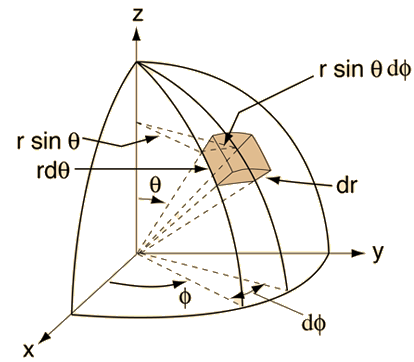
\includegraphics[height=4cm]{sphcoordel}
    %\caption{}
    \label{sphcoordel}
  \end{figure}
\end{frame}

\begin{frame}{Evaluation of the integral}
  Integration over $\phi$

  % \only<>{
  % \begin{equation*}
  %   F(\valk, \vecr) =
  %   \frac{1}{8 \pi^3} \int_{\valk = 0}^{\valk_F} \int_{\theta = 0}^{\pi} \int_{\phi = 0}^{2 \pi}
  %   e^{- i \text{k}r\cos{\theta}}\text{k}^2\sin{\theta} \: d \phi d\theta d \text{k}
  % \end{equation*}
  % }

  \only<1>{
  \begin{equation*}
    F(\valk, \vecr) =
    \frac{1}{8 \pi^3} \int_{\valk = 0}^{\valk_F} \int_{\theta = 0}^{\pi}
    \textcolor{red}{\int_{\phi = 0}^{2 \pi}}
    e^{- i \text{k}r\cos{\theta}}\text{k}^2\sin{\theta} \: \textcolor{red}{d \phi} d\theta d \text{k}
  \end{equation*}
  }

  \only<1>{
  \begin{equation*}
    F(\valk, \vecr) =
    \frac{1}{4 \pi^2} \int_{\valk = 0}^{\valk_F} \int_{\theta = 0}^{\pi}
    e^{- i \text{k}r\cos{\theta}}\text{k}^2\sin{\theta} \: d\theta d \text{k}
  \end{equation*}
  }

\end{frame}

\begin{frame}{Evaluation of the integral}
  Integration over $\theta$

  \only<1,2>{
  \begin{equation*}
    F(\valk, \vecr) =
    \frac{1}{4 \pi^2} \int_{\valk = 0}^{\valk_F} \textcolor{red}{\int_{\theta = 0}^{\pi}}
    e^{- i \text{k}r\textcolor{red}{\cos{\theta}}}\text{k}^2
    \textcolor{red}{\sin{\theta} \: d\theta} d \text{k}
  \end{equation*}
  }

  \only<1,2>{
  \begin{equation*}
    F(\valk, \vecr) =
    \frac{1}{4 \pi^2} \int_{\valk = 0}^{\valk_F} \textcolor{red}{\int_{\theta = 0}^{\pi}}
    e^{- i \text{k}r\textcolor{red}{\cos{\theta}}}\text{k}^2 \: \textcolor{red}{-d\cos{\theta}} d \text{k}
  \end{equation*}
  }

  \only<1>{
  \begin{equation*}
    F(\valk, \vecr) =
    \frac{1}{4 \pi^2} \int_{\valk = 0}^{\valk_F} \textcolor{red}{\int_{\eta = -1}^{1}}
    e^{i \text{k}r\textcolor{red}{\eta}}\text{k}^2 \: \textcolor{red}{d\eta} d \text{k}
  \end{equation*}
  }

  \only<2>{
  \begin{equation*}
    F(\valk, \vecr) =
    \frac{1}{4 \pi^2} \int_{\valk = 0}^{\valk_F}
    \frac{2}{\text{k}r}\sin{(\text{k}r)} \: \text{k}^2 \: d \text{k}
  \end{equation*}
  }

\end{frame}

\begin{frame}[t]{Evaluation of the integral}
  \vspace{0.3cm}
  Integration over k

  \begin{equation*}
    F(\valk, \vecr) =
    \frac{1}{4 \pi^2} \int_{\valk = 0}^{\valk_F}
    \frac{2}{\text{k}r}\sin{(\text{k}r)} \: \text{k}^2 \: d \text{k} =
    \frac{1}{2 \pi^2 r^3} \int_{\valk = 0}^{\valk_F}
    \sin{(\text{k}r)} \: \text{k} r \: d \text{k}r
  \end{equation*}

  \only<1>{
  \begin{equation*}
    F(\valk, \vecr) =
    \frac{1}{2 \pi^2 r^3} \left \{ \sin(\valk_F r) - \valk_F r \cos(\valk_F r) \right \}
  \end{equation*}
  }

  \only<2>{
  \begin{equation*}
    F(\valk, \vecr) =
    \frac{\valk_F^3}{2 \pi^2 r^3 \valk_F^3} \left \{ \sin(\valk_F r) - \valk_F r \cos(\valk_F r) \right \}
  \end{equation*}

  \begin{block}{Fermi wavenumber}
    $$ \valk_F^3 = \frac{3 \pi^2 N}{\V}$$
  \end{block}
  }
\end{frame}

\begin{frame}{Evaluation of the integral}
  \begin{equation*}
    \frac{1}{\mathcal{V}} \sum_{\veck} e^{- i \textbf{k}\vecr}
    \bra{g} \hat c^{\dagger}_{\textbf{k}\sigma} \hat c_{\textbf{k}\sigma} \ket{g} =
    \left ( \frac{N}{2\mathcal{V}} \right )
    \frac{3 \left \{ \sin(\valk_F r) - \valk_F r \cos(\valk_F r) \right \} }{(k_F r)^3}
  \end{equation*}

  \vspace{1cm}
  No divergence at zero: at $\valk_F r \to 0 \iff r \ll \lambda_F$
  \begin{equation*}
    3 \frac{\sin(k_F r) - k_F r \cos(k_F r)}{(k_F r)^3} \approx
    3 \frac{x - x^3/6 - x (1 - x^2/2)}{x^3} = \frac{3}{3} = 1
  \end{equation*}
\end{frame}


\begin{frame}[t]{Bringing it together}
\only<1>{
  \begin{equation*}
        \begin{gathered}
      \rho(\x', \sigma) = -\frac{1}{\V^2}
      \sum_{\veck}
      \bra{g} \hat{c}_{\veck\sigma}^{\dagger} \hat{c}_{\textbf{k}\sigma}\ket{g}e^{i\vec{k}\cdot(\x-\x')} \sum_{\textbf{l}}\bra{g} \hat{c}_{\textbf{l}\sigma}^\dagger  \hat{c}_{\textbf{l}\sigma} \ket{g}
      e^{i\vec{l}\cdot(\x'-\x)}
    \end{gathered}
  \end{equation*}

  \begin{equation*}
    \frac{1}{\mathcal{V}} \sum_{\veck} e^{- i \textbf{k}\vecr}
    \bra{g} \hat c^{\dagger}_{\textbf{k}\sigma} \hat c_{\textbf{k}\sigma} \ket{g} =
    \left ( \frac{N}{2\mathcal{V}} \right )
    \frac{3 \left \{ \sin(\valk_F r) - \valk_F r \cos(\valk_F r) \right \} }{(k_F r)^3}
  \end{equation*}
}

\only<2,3>{
  \begin{equation*}
    \begin{gathered}
      \rho(\x', \sigma) = -\frac{1}{\V^2}
      \textcolor{red}{\sum_{\veck}
      \bra{g} \hat{c}_{\veck\sigma}^{\dagger} \hat{c}_{\textbf{k}\sigma}\ket{g}e^{i\vec{k}\cdot(\x-\x')}} \textcolor{blue}{ \sum_{\textbf{l}}\bra{g} \hat{c}_{\textbf{l}\sigma}^\dagger  \hat{c}_{\textbf{l}\sigma} \ket{g}
      e^{i\vec{l}\cdot(\x'-\x)}}
    \end{gathered}
  \end{equation*}

  \begin{equation*}
    \frac{1}{\mathcal{V}} \sum_{\veck} e^{- i \textbf{k}\vecr}
    \bra{g} \hat c^{\dagger}_{\textbf{k}\sigma} \hat c_{\textbf{k}\sigma} \ket{g} =
    \left ( \frac{N}{2\mathcal{V}} \right )
    \frac{3 \left \{ \sin(\valk_F r) - \valk_F r \cos(\valk_F r) \right \} }{(k_F r)^3}
  \end{equation*}
}
\only<3>{
  \begin{equation}
  	\rho(\x', \sigma) = \left ( \frac{N}{2\mathcal{V}} \right )^2
    \left(\frac{3 \left \{ \sin(\valk_F r) - \valk_F r \cos(\valk_F r) \right \} }{(k_F r)^3}\right)^2
  \end{equation}
}

\end{frame}

\begin{frame}{Bringing it all together}
\only<1>{
\begin{equation*}
\left(\frac{N}{2\V}\right)^2 g_{\sigma\sigma}(\x - \x') = \left(\frac{N}{2\V}\right)^2 - \delta_{\sigma\sigma'} \left ( \frac{N}{2\mathcal{V}} \right )^2
    \left(\frac{3 \left \{ \sin(\valk_F r) - \valk_F r \cos(\valk_F r) \right \} }{(k_F r)^3}\right)^2
\end{equation*}
}
\only<2>{
\begin{equation*}
g_{\sigma\sigma}(\x - \x') = 1 - \delta_{\sigma\sigma'} \left(\frac{3 \left \{ \sin(\valk_F r) - \valk_F r \cos(\valk_F r) \right \} }{(k_F r)^3}\right)^2
\end{equation*}
}
\end{frame}


\begin{frame}{Visualization}
\begin{figure}
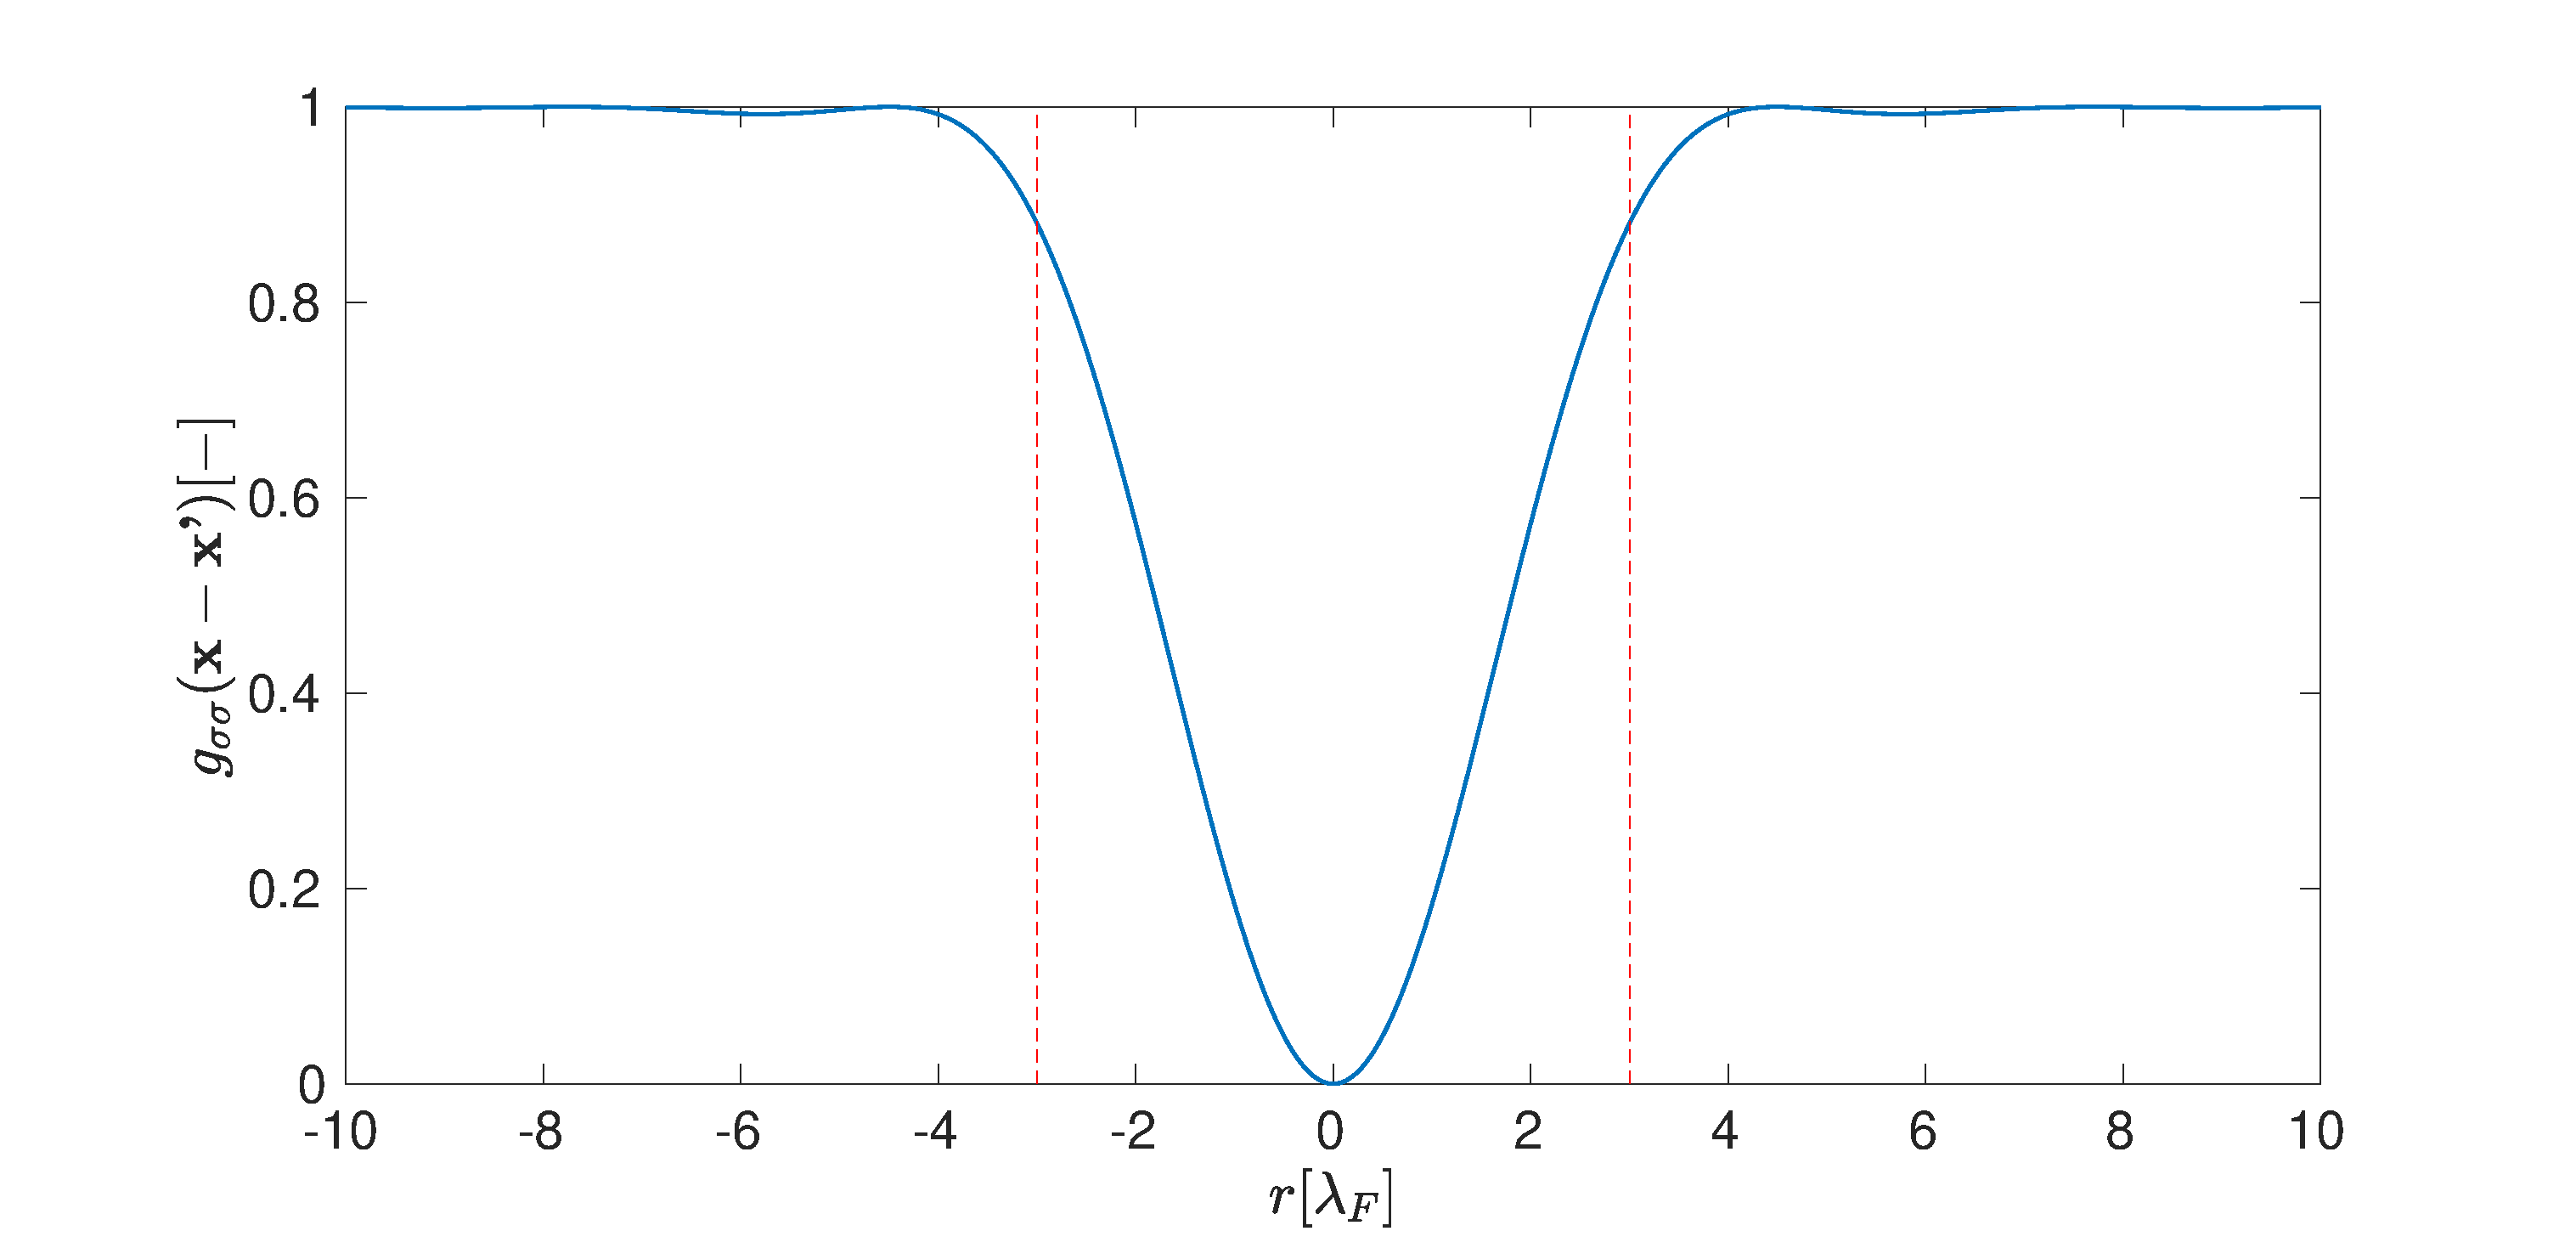
\includegraphics[width=\textwidth]{images/Density}
\end{figure}
\end{frame}
\end{document}
